% ===========================================================================
%  TikuOS — TikuKits DS: Bitmap for Embedded Systems
%  Beamer Presentation
% ===========================================================================
\documentclass[aspectratio=169, 10pt]{beamer}

% ---- Theme ----------------------------------------------------------------
\usetheme{Madrid}
\usecolortheme{whale}
\setbeamertemplate{navigation symbols}{}
\setbeamertemplate{footline}{%
  \leavevmode\hbox{%
    \begin{beamercolorbox}[wd=.33\paperwidth,ht=2.5ex,dp=1ex,center]{author in head/foot}%
      \usebeamerfont{author in head/foot}\insertshortauthor
    \end{beamercolorbox}%
    \begin{beamercolorbox}[wd=.34\paperwidth,ht=2.5ex,dp=1ex,center]{title in head/foot}%
      \usebeamerfont{title in head/foot}\insertshorttitle
    \end{beamercolorbox}%
    \begin{beamercolorbox}[wd=.33\paperwidth,ht=2.5ex,dp=1ex,right]{date in head/foot}%
      \usebeamerfont{date in head/foot}\insertshortdate{}\hspace*{2em}%
      \insertframenumber{}/\inserttotalframenumber\hspace*{2ex}
    \end{beamercolorbox}}%
  \vskip0pt%
}

% ---- Packages -------------------------------------------------------------
\usepackage{listings}
\usepackage{graphicx}
\usepackage{hyperref}
\usepackage{booktabs}
\usepackage{multirow}
\usepackage{tikz}
\usetikzlibrary{arrows.meta, positioning, shapes.geometric, calc,
                decorations.pathreplacing, fit}
\usepackage{amsmath}

% ---- Code listing style ---------------------------------------------------
\lstset{
  basicstyle=\ttfamily\scriptsize,
  keywordstyle=\color{blue}\bfseries,
  commentstyle=\color{gray},
  stringstyle=\color{red!70!black},
  showstringspaces=false,
  breaklines=true,
  frame=single,
  rulecolor=\color{black!30},
  backgroundcolor=\color{blue!3},
  tabsize=4,
}
\lstdefinestyle{cstyle}{
  language=C,
  morekeywords={uint8_t,uint16_t,uint32_t,int32_t,
                tiku_kits_ds_elem_t,
                TIKU_KITS_DS_OK,TIKU_KITS_DS_ERR_NULL,
                TIKU_KITS_DS_ERR_PARAM,TIKU_KITS_DS_ERR_BOUNDS,
                TIKU_KITS_DS_ERR_NOTFOUND,
                TIKU_KITS_DS_BITMAP_MAX_BITS,
                TIKU_KITS_DS_BITMAP_MAX_WORDS,
                NULL,size_t},
}

% ---- Metadata -------------------------------------------------------------
\title[TikuKits DS]{TikuKits DS: Bitmap for Embedded Systems}
\subtitle{Simple. Ubiquitous. Intelligence, Everywhere.}
\author[Ambuj Varshney]{Ambuj Varshney \\ \texttt{ambuj@tiku-os.org}}
\date{\today}

% ===========================================================================
\begin{document}

% ---------------------------------------------------------------------------
\begin{frame}
\titlepage
\end{frame}

% ---------------------------------------------------------------------------
\begin{frame}{Outline}
\tableofcontents
\end{frame}

% ===========================================================================
\section{Motivation}
% ===========================================================================

\begin{frame}{Why a Bitmap on MCUs?}
\begin{columns}[T]
\begin{column}{0.48\textwidth}
\begin{block}{Embedded Use Cases}
\begin{itemize}
  \item \textbf{Sensor active flags} --- 32 sensors in 1 \texttt{uint32\_t}
  \item \textbf{Memory block allocator} --- track free/used blocks
  \item \textbf{Peripheral status} --- which peripherals are enabled
  \item \textbf{GPIO state tracking} --- port pin masks
  \item \textbf{Task ready flags} --- which tasks are runnable
\end{itemize}
\end{block}

\begin{block}{Constraints}
\begin{itemize}
  \item RAM is scarce (2--8\,KB)
  \item Need to track hundreds of boolean flags
  \item Must be efficient --- no wasting a byte per flag
  \item Fast set/clear/test operations
\end{itemize}
\end{block}
\end{column}

\begin{column}{0.48\textwidth}
\begin{center}
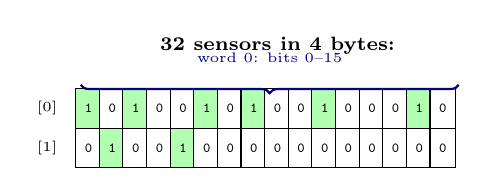
\begin{tikzpicture}[
    >=Stealth,
    bit/.style={draw, minimum width=0.3cm, minimum height=0.5cm,
                font=\tiny\ttfamily}
  ]
  % Show a 32-bit word with some bits set
  \node[font=\scriptsize\bfseries] at (2.4, 0.8) {32 sensors in 4 bytes:};
  \foreach \x/\v/\c in {
    0/1/green!30, 1/0/white, 2/1/green!30, 3/0/white,
    4/0/white, 5/1/green!30, 6/0/white, 7/1/green!30,
    8/0/white, 9/0/white, 10/1/green!30, 11/0/white,
    12/0/white, 13/0/white, 14/1/green!30, 15/0/white} {
    \node[bit, fill=\c] (b\x) at (\x*0.3, 0) {\v};
  }
  \foreach \x/\v/\c in {
    0/0/white, 1/1/green!30, 2/0/white, 3/0/white,
    4/1/green!30, 5/0/white, 6/0/white, 7/0/white,
    8/0/white, 9/0/white, 10/0/white, 11/0/white,
    12/0/white, 13/0/white, 14/0/white, 15/0/white} {
    \node[bit, fill=\c] (c\x) at (\x*0.3, -0.5) {\v};
  }

  \node[font=\tiny, left=0.1cm of b0] {[0]};
  \node[font=\tiny, left=0.1cm of c0] {[1]};

  % Annotation
  \draw[decorate, decoration={brace, amplitude=3pt},
        thick, blue!50!black]
    (4.7, 0.3) -- (-0.1, 0.3)
    node[midway, above=0.15cm, font=\tiny] {word 0: bits 0--15};
\end{tikzpicture}
\end{center}

\vspace{0.5em}
\begin{alertblock}{Extreme RAM Efficiency}
256 boolean flags = 32 bytes (8 \texttt{uint32\_t} words).\\
Using a \texttt{uint8\_t} array: 256 bytes.\\
\textbf{8$\times$ more efficient} with the bitmap.
\end{alertblock}

\vspace{0.3em}
\begin{block}{Bit Operations}
\texttt{set}: OR with mask\\
\texttt{clear}: AND with complement\\
\texttt{toggle}: XOR with mask
\end{block}
\end{column}
\end{columns}
\end{frame}

% ===========================================================================
\section{Architecture}
% ===========================================================================

\begin{frame}{Bit Layout: Words and Positions}
\begin{columns}[T]
\begin{column}{0.48\textwidth}
\textbf{Bit addressing:}
\[
  \text{word index} = N \div 32
\]
\[
  \text{bit position} = N \bmod 32
\]

\vspace{0.5em}
\textbf{Example:} Bit 42\\
$42 \div 32 = 1$ (word index)\\
$42 \bmod 32 = 10$ (bit position within word 1)\\
$\Rightarrow$ \texttt{words[1]} bit 10

\vspace{0.5em}
\begin{block}{Operations via Bit Masks}
\begin{tabular}{@{}ll@{}}
\textbf{Set:}    & \texttt{words[w] |= (1u << pos)} \\
\textbf{Clear:}  & \texttt{words[w] \&= \textasciitilde(1u << pos)} \\
\textbf{Toggle:} & \texttt{words[w] \textasciicircum= (1u << pos)} \\
\textbf{Test:}   & \texttt{(words[w] >> pos) \& 1u} \\
\end{tabular}
\end{block}
\end{column}

\begin{column}{0.48\textwidth}
\begin{center}
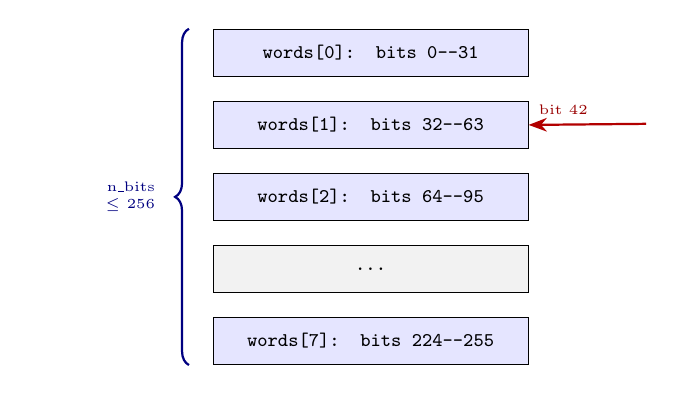
\begin{tikzpicture}[
    >=Stealth,
    word/.style={draw, minimum width=4cm, minimum height=0.6cm,
                 font=\scriptsize\ttfamily}
  ]
  \node[word, fill=blue!10] (w0) {words[0]: bits 0--31};
  \node[word, fill=blue!10, below=0.3cm of w0] (w1) {words[1]: bits 32--63};
  \node[word, fill=blue!10, below=0.3cm of w1] (w2) {words[2]: bits 64--95};
  \node[word, fill=gray!10, below=0.3cm of w2] (wd) {...};
  \node[word, fill=blue!10, below=0.3cm of wd] (wn)
    {words[7]: bits 224--255};

  % Highlight bit 42
  \draw[->, thick, red!70!black] (3.5, -0.9) -- (w1.east)
    node[above right, font=\tiny, text=red!60!black] {bit 42};

  % Brace for n_bits
  \draw[decorate, decoration={brace, amplitude=5pt, mirror},
        thick, blue!50!black]
    ([xshift=-0.3cm]w0.north west) -- ([xshift=-0.3cm]wn.south west)
    node[midway, left=0.3cm, font=\tiny, text=blue!50!black,
         text width=1.5cm, align=right] {n\_bits\\$\leq$ 256};
\end{tikzpicture}
\end{center}

\vspace{0.3em}
\begin{alertblock}{Non-Word-Aligned Sizes}
For $n = 50$ bits: 2 words needed.\\
\texttt{set\_all()} masks the partial last word to avoid setting bits
beyond $n$: \texttt{(1u << 18) - 1} for the upper 18 bits of word 1.
\end{alertblock}
\end{column}
\end{columns}
\end{frame}

% ===========================================================================
\section{Data Structure}
% ===========================================================================

\begin{frame}[fragile]{The \texttt{tiku\_kits\_ds\_bitmap} Structure}
\begin{columns}[T]
\begin{column}{0.48\textwidth}
\begin{lstlisting}[style=cstyle,
  title={ds/bitmap/tiku\_kits\_ds\_bitmap.h}]
#define TIKU_KITS_DS_BITMAP_MAX_BITS 256

#define TIKU_KITS_DS_BITMAP_MAX_WORDS \
    ((TIKU_KITS_DS_BITMAP_MAX_BITS \
      + 31) / 32)

struct tiku_kits_ds_bitmap {
    uint32_t words[
        TIKU_KITS_DS_BITMAP_MAX_WORDS];
    uint16_t n_bits;
};
\end{lstlisting}

\vspace{0.3em}
\textbf{Memory footprint} (default config):\\
$8 \times 4 + 2 = 34$ bytes for 256 bits.\\
That is 256 boolean flags in 34 bytes total.
\end{column}

\begin{column}{0.48\textwidth}
\begin{block}{Design Properties}
\begin{itemize}
  \item \textbf{Packed storage:} 32 bits per \texttt{uint32\_t} word
  \item \textbf{Static allocation:} compile-time maximum size
  \item \textbf{Runtime sizing:} \texttt{n\_bits} can be $\leq$ MAX\_BITS
  \item \textbf{Word-aligned ops:} all operations use 32-bit masks
\end{itemize}
\end{block}

\vspace{0.3em}
\begin{table}
\centering
\scriptsize
\begin{tabular}{@{}rrr@{}}
\toprule
\textbf{Max Bits} & \textbf{Words} & \textbf{RAM (bytes)} \\
\midrule
32  & 1  & 6 \\
64  & 2  & 10 \\
128 & 4  & 18 \\
256 & 8  & 34 \\
\bottomrule
\end{tabular}
\end{table}
\end{column}
\end{columns}
\end{frame}

% ===========================================================================
\section{API Reference}
% ===========================================================================

\begin{frame}[fragile]{Complete API}
\begin{table}
\centering
\small
\begin{tabular}{@{}lp{7.5cm}@{}}
\toprule
\textbf{Function} & \textbf{Description} \\
\midrule
\texttt{tiku\_kits\_ds\_bitmap\_init(bm, n)}
  & Initialize with \texttt{n} bits, all cleared to 0 \\
\midrule
\texttt{tiku\_kits\_ds\_bitmap\_set(bm, bit)}
  & Set bit to 1 (OR with mask) \\
\texttt{tiku\_kits\_ds\_bitmap\_clear\_bit(bm, bit)}
  & Clear bit to 0 (AND with complement) \\
\texttt{tiku\_kits\_ds\_bitmap\_toggle(bm, bit)}
  & Flip bit (XOR with mask) \\
\texttt{tiku\_kits\_ds\_bitmap\_test(bm, bit, \&result)}
  & Test if bit is set; result = 0 or 1 \\
\midrule
\texttt{tiku\_kits\_ds\_bitmap\_set\_all(bm)}
  & Set all valid bits to 1 \\
\texttt{tiku\_kits\_ds\_bitmap\_clear\_all(bm)}
  & Clear all bits to 0 \\
\midrule
\texttt{tiku\_kits\_ds\_bitmap\_count\_set(bm)}
  & Count of bits that are 1 (popcount) \\
\texttt{tiku\_kits\_ds\_bitmap\_count\_clear(bm)}
  & Count of bits that are 0 ($n - \text{popcount}$) \\
\midrule
\texttt{tiku\_kits\_ds\_bitmap\_find\_first\_set(bm, \&bit)}
  & Index of lowest set bit \\
\texttt{tiku\_kits\_ds\_bitmap\_find\_first\_clear(bm, \&bit)}
  & Index of lowest clear bit \\
\bottomrule
\end{tabular}
\end{table}
\end{frame}

% ===========================================================================
\section{Configuration}
% ===========================================================================

\begin{frame}[fragile]{Compile-Time Configuration}
\begin{columns}[T]
\begin{column}{0.48\textwidth}
\begin{lstlisting}[style=cstyle,
  title={Configurable parameters}]
/* Maximum number of bits */
#ifndef TIKU_KITS_DS_BITMAP_MAX_BITS
#define TIKU_KITS_DS_BITMAP_MAX_BITS 256
#endif

/* Derived: number of 32-bit words */
#define TIKU_KITS_DS_BITMAP_MAX_WORDS \
    ((TIKU_KITS_DS_BITMAP_MAX_BITS \
      + 31) / 32)
\end{lstlisting}

\vspace{0.3em}
\begin{block}{Shared Return Codes}
\begin{itemize}
  \item \texttt{TIKU\_KITS\_DS\_OK} (0)
  \item \texttt{TIKU\_KITS\_DS\_ERR\_NULL} ($-1$)
  \item \texttt{TIKU\_KITS\_DS\_ERR\_PARAM} ($-4$)
  \item \texttt{TIKU\_KITS\_DS\_ERR\_BOUNDS} ($-6$)
  \item \texttt{TIKU\_KITS\_DS\_ERR\_NOTFOUND} ($-5$)
\end{itemize}
\end{block}
\end{column}

\begin{column}{0.48\textwidth}
\begin{lstlisting}[style=cstyle,
  title={Runtime initialization}]
struct tiku_kits_ds_bitmap bm;

/* 64 bits = 2 words = 10 bytes */
tiku_kits_ds_bitmap_init(&bm, 64);

/* Or for 32 sensor flags */
tiku_kits_ds_bitmap_init(&bm, 32);

/* Compile-time override: */
/* -DTIKU_KITS_DS_BITMAP_MAX_BITS=512 */
\end{lstlisting}

\vspace{0.3em}
\begin{alertblock}{Bounds Checking}
Every single-bit operation validates
\texttt{bit < n\_bits} and returns
\texttt{ERR\_BOUNDS} on out-of-range access.
No silent corruption.
\end{alertblock}
\end{column}
\end{columns}
\end{frame}

% ===========================================================================
\section{Bit Operations}
% ===========================================================================

\begin{frame}[fragile]{Set, Clear, Toggle, Test}
\begin{columns}[T]
\begin{column}{0.48\textwidth}
\begin{lstlisting}[style=cstyle,
  title={Set --- OR with mask}]
int tiku_kits_ds_bitmap_set(
    struct tiku_kits_ds_bitmap *bm,
    uint16_t bit)
{
    uint16_t w   = bit / 32;
    uint16_t pos = bit % 32;
    bm->words[w] |=
        ((uint32_t)1u << pos);
    return TIKU_KITS_DS_OK;
}
\end{lstlisting}

\begin{lstlisting}[style=cstyle,
  title={Clear --- AND with complement}]
int tiku_kits_ds_bitmap_clear_bit(
    struct tiku_kits_ds_bitmap *bm,
    uint16_t bit)
{
    uint16_t w   = bit / 32;
    uint16_t pos = bit % 32;
    bm->words[w] &=
        ~((uint32_t)1u << pos);
    return TIKU_KITS_DS_OK;
}
\end{lstlisting}
\end{column}

\begin{column}{0.48\textwidth}
\begin{lstlisting}[style=cstyle,
  title={Toggle --- XOR with mask}]
int tiku_kits_ds_bitmap_toggle(
    struct tiku_kits_ds_bitmap *bm,
    uint16_t bit)
{
    uint16_t w   = bit / 32;
    uint16_t pos = bit % 32;
    bm->words[w] ^=
        ((uint32_t)1u << pos);
    return TIKU_KITS_DS_OK;
}
\end{lstlisting}

\begin{lstlisting}[style=cstyle,
  title={Test --- shift and mask}]
int tiku_kits_ds_bitmap_test(
    const struct tiku_kits_ds_bitmap *bm,
    uint16_t bit, uint8_t *result)
{
    uint16_t w   = bit / 32;
    uint16_t pos = bit % 32;
    *result = (uint8_t)
        ((bm->words[w] >> pos) & 1u);
    return TIKU_KITS_DS_OK;
}
\end{lstlisting}
\end{column}
\end{columns}
\end{frame}

% ===========================================================================
\section{Kernighan Popcount}
% ===========================================================================

\begin{frame}[fragile]{Counting Set Bits: Kernighan's Method}
\begin{columns}[T]
\begin{column}{0.48\textwidth}
\begin{lstlisting}[style=cstyle,
  title={popcount32 --- count set bits in a word}]
static uint16_t popcount32(uint32_t n)
{
    uint16_t count = 0;

    while (n) {
        n &= (n - 1);
        count++;
    }
    return count;
}
\end{lstlisting}

\begin{lstlisting}[style=cstyle,
  title={count\_set --- sum across all words}]
uint16_t tiku_kits_ds_bitmap_count_set(
    const struct tiku_kits_ds_bitmap *bm)
{
    uint16_t n_words, count, i;
    n_words = (bm->n_bits + 31) / 32;
    count = 0;
    for (i = 0; i < n_words; i++) {
        count += popcount32(bm->words[i]);
    }
    return count;
}
\end{lstlisting}
\end{column}

\begin{column}{0.48\textwidth}
\textbf{How \texttt{n \&= (n - 1)} works:}

\vspace{0.3em}
Each iteration clears the \textbf{lowest set bit}:
\begin{center}
\begin{tabular}{@{}rll@{}}
\toprule
\textbf{Step} & \textbf{n (binary)} & \textbf{Action} \\
\midrule
0 & \texttt{1010 1100} & start \\
1 & \texttt{1010 1000} & clear bit 2 \\
2 & \texttt{1010 0000} & clear bit 3 \\
3 & \texttt{1000 0000} & clear bit 5 \\
4 & \texttt{0000 0000} & clear bit 7, done \\
\bottomrule
\end{tabular}
\end{center}

\vspace{0.5em}
\begin{block}{Why Kernighan?}
\begin{itemize}
  \item Loop runs \textbf{once per set bit}, not per total bit
  \item For sparse bitmaps (few flags set): very fast
  \item No lookup table needed (saves FRAM/Flash)
  \item Works on any word size
\end{itemize}
\end{block}

\textbf{Worst case:} all 32 bits set $\Rightarrow$ 32 iterations.\\
\textbf{Best case:} no bits set $\Rightarrow$ 0 iterations.
\end{column}
\end{columns}
\end{frame}

% ===========================================================================
\section{Find First Set / Clear}
% ===========================================================================

\begin{frame}[fragile]{Find First Set and Find First Clear}
\begin{columns}[T]
\begin{column}{0.48\textwidth}
\begin{lstlisting}[style=cstyle,
  title={find\_first\_set --- lowest set bit}]
int tiku_kits_ds_bitmap_find_first_set(
    const struct tiku_kits_ds_bitmap *bm,
    uint16_t *bit)
{
    uint16_t n_words, i, pos, idx;
    uint32_t w;

    n_words = (bm->n_bits + 31) / 32;
    for (i = 0; i < n_words; i++) {
        w = bm->words[i];
        if (w == 0) continue;

        /* Find lowest set bit */
        pos = 0;
        while ((w & 1u) == 0) {
            w >>= 1;
            pos++;
        }
        idx = (uint16_t)(i * 32u + pos);
        if (idx < bm->n_bits) {
            *bit = idx;
            return TIKU_KITS_DS_OK;
        }
    }
    return TIKU_KITS_DS_ERR_NOTFOUND;
}
\end{lstlisting}
\end{column}

\begin{column}{0.48\textwidth}
\textbf{Find first clear} uses the same algorithm
on the \textbf{inverted} word (\texttt{\textasciitilde bm->words[i]}).

\vspace{0.5em}
\begin{block}{Use Case: Memory Block Allocator}
\begin{enumerate}
  \item Each bit represents a memory block
  \item \texttt{find\_first\_clear()} $\rightarrow$ next free block
  \item \texttt{set(bit)} $\rightarrow$ mark block as allocated
  \item \texttt{clear\_bit(bit)} $\rightarrow$ free the block
\end{enumerate}
\end{block}

\vspace{0.5em}
\begin{alertblock}{Boundary Safety}
The function checks \texttt{idx < n\_bits} to avoid
reporting bits in the padding zone of the last word
(for non-word-aligned sizes like 50 bits).
\end{alertblock}
\end{column}
\end{columns}
\end{frame}

% ===========================================================================
\section{Examples}
% ===========================================================================

\begin{frame}[fragile]{Example 1: Sensor Active Flags}
\begin{lstlisting}[style=cstyle,
  title={Track which sensors are active using a bitmap}]
#define SENSOR_TEMP     0
#define SENSOR_HUMID    1
#define SENSOR_LIGHT    2
#define SENSOR_ACCEL    3
#define SENSOR_GYRO     4
#define NUM_SENSORS     32

struct tiku_kits_ds_bitmap sensor_flags;
uint8_t is_active;
uint16_t active_count;

tiku_kits_ds_bitmap_init(&sensor_flags, NUM_SENSORS);

/* Enable specific sensors */
tiku_kits_ds_bitmap_set(&sensor_flags, SENSOR_TEMP);
tiku_kits_ds_bitmap_set(&sensor_flags, SENSOR_LIGHT);
tiku_kits_ds_bitmap_set(&sensor_flags, SENSOR_ACCEL);

/* Check if a sensor is active */
tiku_kits_ds_bitmap_test(&sensor_flags, SENSOR_GYRO, &is_active);
/* is_active == 0 (gyro not enabled) */

/* How many sensors are active? */
active_count = tiku_kits_ds_bitmap_count_set(&sensor_flags);
/* active_count == 3 */
\end{lstlisting}
\end{frame}

% ---------------------------------------------------------------------------
\begin{frame}[fragile]{Example 2: Memory Block Allocator}
\begin{columns}[T]
\begin{column}{0.52\textwidth}
\begin{lstlisting}[style=cstyle,
  title={Simple block allocator with bitmap}]
#define NUM_BLOCKS 64  /* 64 blocks */
#define BLOCK_SIZE 32  /* 32 bytes each */

struct tiku_kits_ds_bitmap blk_map;
uint8_t buffer[NUM_BLOCKS * BLOCK_SIZE];

tiku_kits_ds_bitmap_init(
    &blk_map, NUM_BLOCKS);

/* Allocate a block */
uint16_t blk;
if (tiku_kits_ds_bitmap_find_first_clear(
        &blk_map, &blk) ==
    TIKU_KITS_DS_OK) {
    tiku_kits_ds_bitmap_set(
        &blk_map, blk);
    /* Use buffer[blk * BLOCK_SIZE] */
}

/* Free a block */
tiku_kits_ds_bitmap_clear_bit(
    &blk_map, blk);

/* Check utilization */
uint16_t used =
    tiku_kits_ds_bitmap_count_set(
        &blk_map);
\end{lstlisting}
\end{column}

\begin{column}{0.44\textwidth}
\begin{center}
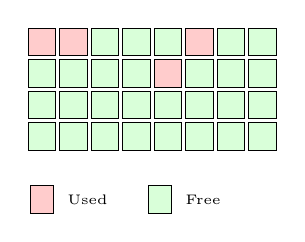
\begin{tikzpicture}[
    >=Stealth,
    blk/.style={draw, minimum width=0.35cm, minimum height=0.35cm,
                font=\tiny\ttfamily}
  ]
  % Show blocks as a grid
  \foreach \y in {0,...,3} {
    \foreach \x in {0,...,7} {
      \pgfmathtruncatemacro{\idx}{\y*8+\x}
      \pgfmathtruncatemacro{\isused}{
        (\idx==0 || \idx==1 || \idx==5 || \idx==12) ? 1 : 0}
      \ifnum\isused=1
        \node[blk, fill=red!20] at (\x*0.4, -\y*0.4) {};
      \else
        \node[blk, fill=green!15] at (\x*0.4, -\y*0.4) {};
      \fi
    }
  }

  % Legend
  \node[blk, fill=red!20, minimum width=0.3cm] at (0, -2.0) {};
  \node[font=\tiny, right] at (0.2, -2.0) {Used};
  \node[blk, fill=green!15, minimum width=0.3cm] at (1.5, -2.0) {};
  \node[font=\tiny, right] at (1.7, -2.0) {Free};
\end{tikzpicture}
\end{center}

\vspace{0.5em}
\begin{block}{Allocator Pattern}
\begin{itemize}
  \item \texttt{find\_first\_clear} $\rightarrow$ $O(n/32)$ scan
  \item \texttt{set} $\rightarrow$ mark allocated
  \item \texttt{clear\_bit} $\rightarrow$ free block
  \item \texttt{count\_set} $\rightarrow$ usage stats
\end{itemize}
64 blocks tracked in just 10 bytes.
\end{block}
\end{column}
\end{columns}
\end{frame}

% ---------------------------------------------------------------------------
\begin{frame}[fragile]{Example 3: Peripheral Status Tracking}
\begin{lstlisting}[style=cstyle,
  title={Track peripheral enable/disable state}]
#define PERIPH_UART0   0
#define PERIPH_SPI0    1
#define PERIPH_I2C0    2
#define PERIPH_ADC     3
#define PERIPH_TIMER0  4
#define PERIPH_TIMER1  5
#define PERIPH_DMA     6
#define NUM_PERIPHS    8

struct tiku_kits_ds_bitmap periph_status;
uint16_t first_on;

tiku_kits_ds_bitmap_init(&periph_status, NUM_PERIPHS);

/* Enable peripherals needed for sensor reading */
tiku_kits_ds_bitmap_set(&periph_status, PERIPH_I2C0);
tiku_kits_ds_bitmap_set(&periph_status, PERIPH_ADC);
tiku_kits_ds_bitmap_set(&periph_status, PERIPH_TIMER0);

/* Enter low-power: disable all, remembering which were on */
/* (save bitmap state, then clear_all) */
tiku_kits_ds_bitmap_clear_all(&periph_status);

/* Toggle a peripheral on wake-up */
tiku_kits_ds_bitmap_toggle(&periph_status, PERIPH_UART0);
\end{lstlisting}
\end{frame}

% ===========================================================================
\section{Bulk Operations}
% ===========================================================================

\begin{frame}[fragile]{Set All and Clear All: Handling Partial Words}
\begin{columns}[T]
\begin{column}{0.48\textwidth}
\begin{lstlisting}[style=cstyle,
  title={set\_all --- masks the last word}]
int tiku_kits_ds_bitmap_set_all(
    struct tiku_kits_ds_bitmap *bm)
{
    uint16_t full_words;
    uint16_t remainder;
    uint16_t i;

    full_words = bm->n_bits / 32;
    remainder  = bm->n_bits % 32;

    /* Full words: all ones */
    for (i = 0; i < full_words; i++) {
        bm->words[i] = 0xFFFFFFFFu;
    }

    /* Partial last word: only valid bits */
    if (remainder > 0) {
        bm->words[full_words] =
            ((uint32_t)1u << remainder)
            - 1u;
    }

    return TIKU_KITS_DS_OK;
}
\end{lstlisting}
\end{column}

\begin{column}{0.48\textwidth}
\textbf{Why mask the last word?}

\vspace{0.3em}
For $n = 50$ bits:
\begin{itemize}
  \item Word 0: bits 0--31 $\rightarrow$ \texttt{0xFFFFFFFF}
  \item Word 1: bits 32--49 $\rightarrow$ only 18 valid bits
  \item Mask: \texttt{(1u << 18) - 1 = 0x0003FFFF}
\end{itemize}

\vspace{0.3em}
If we set all 32 bits of word 1, \texttt{count\_set()} would
return 64 instead of 50 --- wrong!

\vspace{0.5em}
\begin{block}{\texttt{clear\_all} is simpler}
Just \texttt{memset(words, 0, ...)}. No masking needed because
extra zero bits in the last word are harmless.
\end{block}

\vspace{0.3em}
\begin{alertblock}{Invariant}
Bits beyond \texttt{n\_bits} are always zero.
\texttt{set\_all()} preserves this invariant.
\end{alertblock}
\end{column}
\end{columns}
\end{frame}

% ===========================================================================
\section{Test Suite}
% ===========================================================================

\begin{frame}{Test Cases Overview}
\begin{table}
\centering
\small
\begin{tabular}{@{}clp{7cm}@{}}
\toprule
\textbf{\#} & \textbf{Test Function} & \textbf{What It Verifies} \\
\midrule
1 & \texttt{test\_kits\_ds\_bitmap\_init}
  & Initialization, all bits zero, parameter validation \\
2 & \texttt{test\_kits\_ds\_bitmap\_set\_clear\_test}
  & Set/clear individual bits, word boundaries, bounds \\
3 & \texttt{test\_kits\_ds\_bitmap\_toggle}
  & Toggle 0$\rightarrow$1$\rightarrow$0, adjacent bits unaffected \\
4 & \texttt{test\_kits\_ds\_bitmap\_set\_all\_clear\_all}
  & Bulk ops with non-word-aligned sizes (50 bits) \\
5 & \texttt{test\_kits\_ds\_bitmap\_count\_set\_clear}
  & Popcount accuracy, idempotent set, clear one \\
6 & \texttt{test\_kits\_ds\_bitmap\_find\_first\_set}
  & Find lowest set bit, empty bitmap returns NOTFOUND \\
7 & \texttt{test\_kits\_ds\_bitmap\_find\_first\_clear}
  & Find lowest clear bit, all-set returns NOTFOUND \\
8 & \texttt{test\_kits\_ds\_bitmap\_boundary\_bits}
  & 33-bit and 1-bit bitmaps, word boundary correctness \\
9 & \texttt{test\_kits\_ds\_bitmap\_null\_inputs}
  & All functions reject NULL with ERR\_NULL \\
\bottomrule
\end{tabular}
\end{table}
\end{frame}

% ===========================================================================
\section{Summary}
% ===========================================================================

\begin{frame}{Summary}
\begin{columns}[T]
\begin{column}{0.48\textwidth}
\begin{block}{What We Built}
\begin{itemize}
  \item Fixed-size bitmap packed into 32-bit words
  \item 256 flags in 34 bytes (8$\times$ more efficient than byte array)
  \item $O(1)$ set/clear/toggle/test per bit
  \item Kernighan popcount for efficient counting
  \item Find-first-set/clear for allocation patterns
\end{itemize}
\end{block}

\begin{block}{Key Design Choices}
\begin{itemize}
  \item 32-bit words for natural alignment
  \item Partial last word masked in \texttt{set\_all}
  \item Kernighan loop: runs per set bit, not per total bit
  \item Bounds checking on every operation
\end{itemize}
\end{block}
\end{column}

\begin{column}{0.48\textwidth}
\begin{block}{Use Cases}
\begin{itemize}
  \item Sensor active flags (32 sensors = 4 bytes)
  \item Memory block allocator bitmap
  \item Peripheral status tracking
  \item GPIO port pin state management
  \item Task ready/sleep flags
\end{itemize}
\end{block}

\begin{block}{Files}
\scriptsize
\begin{tabular}{@{}lp{4.5cm}@{}}
Header: & \texttt{ds/bitmap/tiku\_kits\_ds\_bitmap.h} \\
Source: & \texttt{ds/bitmap/tiku\_kits\_ds\_bitmap.c} \\
Tests: & \texttt{tests/ds/test\_kits\_ds\_bitmap.c} \\
Common: & \texttt{ds/tiku\_kits\_ds.h} \\
\end{tabular}
\end{block}
\end{column}
\end{columns}
\end{frame}

% ---------------------------------------------------------------------------
\begin{frame}{Thank You}
\begin{center}
\Large\textbf{TikuKits DS: Bitmap}\\[0.5em]
\normalsize Compact Boolean Flag Storage for Physical AI Endpoints\\[1.5em]

\begin{tabular}{rl}
  Repository: & \url{https://github.com/tikuos/tikuOS} \\
  License:    & Apache 2.0 \\
  Common:     & \texttt{tikukits/ds/tiku\_kits\_ds.h} \\
  Header:     & \texttt{tikukits/ds/bitmap/tiku\_kits\_ds\_bitmap.h} \\
  Source:     & \texttt{tikukits/ds/bitmap/tiku\_kits\_ds\_bitmap.c} \\
  Tests:      & \texttt{tikukits/tests/ds/test\_kits\_ds\_bitmap.c} \\
\end{tabular}
\end{center}
\end{frame}

\end{document}
